\documentclass[compress]{beamer}
\mode<presentation>

\usetheme{Warsaw}
\definecolor{innotek}{RGB}{2,52,173}
\setbeamercolor*{palette primary}{use=structure,fg=white,bg=innotek}
%\usecolortheme[RGB={2,52,173}]{structure}
\defbeamertemplate*{footline}{shadow theme}
{%
  \leavevmode%
  \hbox{\begin{beamercolorbox}[wd=.5\paperwidth,ht=2.5ex,dp=1.125ex,leftskip=.3cm plus1fil,rightskip=.3cm]{author in head/foot}%
    \usebeamerfont{author in head/foot}\hfill\insertshortauthor%
  \end{beamercolorbox}%
  \begin{beamercolorbox}[wd=.5\paperwidth,ht=2.5ex,dp=1.125ex,leftskip=.3cm,rightskip=.3cm plus1fil]{title in head/foot}%
      \usebeamerfont{title in head/foot}\insertshorttitle\hfill\insertframenumber\,/\,\inserttotalframenumber%
  \end{beamercolorbox}}%
  \vskip0pt%
}
\setbeamertemplate{navigation symbols}{}%remove navigation symbols

\usepackage{subfigure}
\usepackage{multicol}
%\usepackage{amsmath}
\usepackage{epsfig}
\usepackage{graphicx}
\usepackage[all,knot]{xy}
\xyoption{arc}
\usepackage{url}
\usepackage{multimedia}
\usepackage{hyperref}
\usepackage{setspace}

% define your own colours:
\definecolor{innotek}{RGB}{1,54,160}
\definecolor{Red}{rgb}{1,0,0}
\definecolor{Blue}{rgb}{0,0,1}
\definecolor{Green}{rgb}{0,1,0}
\definecolor{magenta}{rgb}{1,0,.6}
\definecolor{lightblue}{rgb}{0,.5,1}
\definecolor{lightpurple}{rgb}{.6,.4,1}
\definecolor{gold}{rgb}{.6,.5,0}
\definecolor{orange}{rgb}{1,0.4,0}
\definecolor{hotpink}{rgb}{1,0,0.5}
\definecolor{newcolor2}{rgb}{.5,.3,.5}
\definecolor{newcolor}{rgb}{0,.3,1}
\definecolor{newcolor3}{rgb}{1,0,.35}
\definecolor{darkgreen1}{rgb}{0, .35, 0}
\definecolor{darkgreen}{rgb}{0, .6, 0}
\definecolor{darkred}{rgb}{.75,0,0}

\xdefinecolor{olive}{cmyk}{0.64,0,0.95,0.4}
\xdefinecolor{purpleish}{cmyk}{0.75,0.75,0,0}

\useoutertheme[subsection=false]{smoothbars}

\title{POW-R}
\subtitle{Power Outlet Wireless Reporter}
\author[]{Grace De Geus\\Charles Hathaway\\Forest Immel\\Nate Pickett\\Niloc Quimby}
\date{April $24^{th}$, 2013}

\begin{document}

\frame{
    \titlepage
}


\subsection{Requirements Summary}
\frame{
\frametitle{Functional Requirements}
}

\frame {
 \frametitle{Satellite Requirements}
\begin{itemize}
 \item Standard NEMA 5-15 mains electrical outlets
 \item Two outlet sockets on the opposite side of the plugs %if it takes up two outlets, it should provide two outlets
 \item Less than 5\% error on readings %current and voltage 
 \item Power draw less than 1W per Satellite
 \item Broadcasts information up to 500M
 \item Transmits every 1.0 seconds
 \item Zigbee compatible
 \item Encrypted communication
\end{itemize}
}

\frame{
\frametitle{Server Requirements}
\begin{itemize}
 \item Physical Server inside the monitored building
 \item Runs on less than 10 W
 \item Hosts web server for Display
 \item Button to connect Satellites
 \item Ability to connect to the user's network
 \item Zigbee compatible
 \item Encrypted communication
\end{itemize}
}

\frame{
\frametitle{Display Requirements}
\begin{itemize}
 \item User Management
 \item Group Management
 \item Device Management
 \item Satellite Management
\end{itemize}
}

\frame{
\frametitle{Display Requirements Cont.}
\begin{itemize}
 \item View Data
	\begin{itemize}
	 \item View Device Power Consumption
		 %Shows the user power consumption on a per-device (or device group) basis
	 \item View Power Consumption Over Time
		 % Shows the user power consumption over a specified range of time
		 % Includes total and per-device power consumption
	 \item View Device Cost Over Time
	%Shows the user the cost to run a device, or group of devices, over a specified time range
		% Shows the user a comparison of device costs over a specified range with a given interval E.g. Show them the device cost every month for the past year
	
	\end{itemize}
\end{itemize}
}

\frame{
 \frametitle{Display Requirements Cont.}
\begin{itemize}	
	\item  Power Bill Guesstimator
	\begin{itemize}
	 \item View cost to run a specified device over a period of time in the future
	 \item View cost to run multiple devices over a period of time
	 \item View expected power bill if a device is added
	 \item Allow the user to specify cost of power for
	 \begin{itemize}
		\item Specific time ranges
		\item Specific power-usage ranges
		 \item E.g. Power cost the user \$0.08 per kW/hr for 
		 	the first 500 kW/hrs, and \$0.10 after that
		\end{itemize}
	\end{itemize}
\end{itemize}
}

\frame{

\frametitle{Non-functional Requirements}
}

\frame{
\frametitle{Satellite Requirements}
\begin{itemize}
 	\item Able to work in groups of up to 255 for any one Server within a 500 meter radius
	\item Conveniently sized and shaped
	\begin{itemize}
		\item Unobtrusive
		\item As small as possible given the hardware
	\end{itemize}
	\item A small LED near each socked to indicate power
	\item A button for turning On or Off
	\item A button to initiate connection to the Server
	\item Will be an unobtrusive color other than white
	\item Data sent from Satellite to Server shall be encrypted
\end{itemize}
}

\frame{
\frametitle{Server Requirements}
\begin{itemize}
	\item Enough hard drive space to hold 5 years of data
	\item Supports up to 255 Satellites
	\item Receives a reading from any Satellite at any time
	\begin{itemize}
		\item Losing readings is considered an error
	\end{itemize}
	\item Hardware specifications:
	\begin{itemize}
		\item 1.2 GHz CPU, i386 architecture
		\item 512 MB Ram
		\item 40G SSD Drive
	\end{itemize}
\end{itemize}
}

\frame{
\frametitle{Server Requirements Cont.}
\begin{itemize}
	\item Small and unobtrusive case
	\item Color shall not be white
	\item User can add Satellites at any time
	\item Encryption used on all communication to Satellites
	\item User cannot log in to the Server and get a shell
\end{itemize}
}


\frame{
\frametitle{Display Requirements}
\begin{itemize}
 	\item Interface is easy to learn
 	\item Maximum of 500 milliseconds to load a page
	\item Data is not lost when a device is moved to a new Satellite
	\item Not vulnerable to SQL injection
	\item Not vulnerable to XSS
	\item No unauthorized access
	\item Data transmitted to the Display is encrypted
\end{itemize}
}

\frame{
\frametitle{Display Requirements Cont.}
\begin{itemize}
	\item User has a modern web browser:
	\begin{itemize}
		\item Internet Explorer 9
		\item Chrome 22
		\item Firefox 15
	\end{itemize}
	\item User's PC can render a page in their web browser that contains:
	\begin{itemize}
		\item Javascript
		\item Images
		\item Extensive mark up
	\end{itemize}
\end{itemize}
}






\section{Architecture}
\section{Software}

\subsection{Overview}

\frame {
 \frametitle{Software Overview}
 \begin{itemize}
  \item Python on the backend
  \begin{enumerate}[A.]
   \item Django for the REST, HTTP stuff
   \item Custom python to interact with Arduino interface
  \end{enumerate}
  \item Heavy Javascript on the frontend
  \begin{enumerate}[A.]
   \item jqplot for creating graphs (jQuery included)
   \item RequireJS for module dependency and loading
   \item BackboneJS for MVC architecture
  \end{enumerate}
 \end{itemize}
}

\frame{
 \frametitle{Backend Overview}
 \begin{itemize}
  \item Django will be used to handle database
  \item Tastypie will be used to prototype the REST API
  \item Django admin will be used to prototype the admin interface
  \item Each functional area of the project will be a Django module
  \begin{enumerate}[A.]
   \item Power Bill Guestimator
   \item Satellite
   \item REST API
  \end{enumerate}
 \end{itemize}
}

\frame{
 \frametitle{Backend Overview}
 \begin{center}
  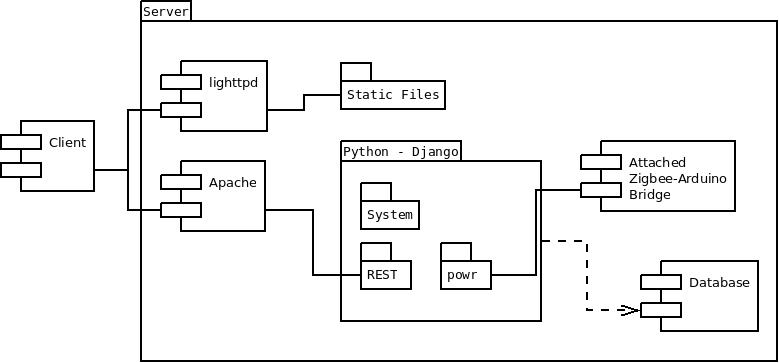
\includegraphics[width=0.8\textwidth]{Diagrams/ServerDependency.jpg}
 \end{center}
}

\frame{
 \frametitle{Frontend Overview}
 \begin{itemize}
  \item RequireJS - Loads all the required modules for each page
  \begin{enumerate}[A.]
   \item Helps keep the scope clean
   \item Enhances modular development
  \end{enumerate}
  \item Backbone.js - MVC Architecture on the client-side
  \item iCanHaz - Provides the 'V' part of MVC
  \item jqplot - Renders charts and graphs
  \item jQuery - Deals with all the behind-the-scenes AJAX stuff
 \end{itemize}
}

\frame{
 \frametitle{Frontend Overview}
 \begin{center}
  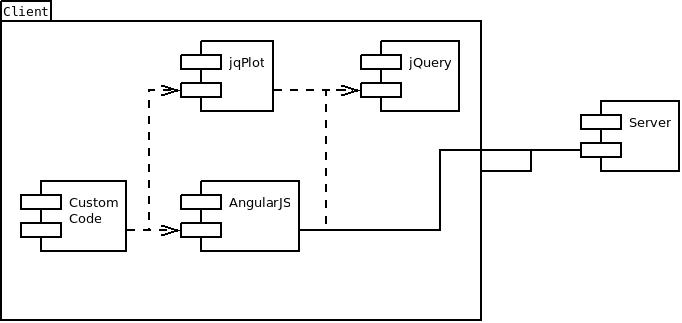
\includegraphics[width=0.8\textwidth]{Diagrams/ClientDependency.jpg}
 \end{center}
}

\subsection{Interesting problems}

\frame{
 \frametitle{Power Bill Guestimator}
 \begin{itemize}
  \item Power companies have different ways of charging
  \begin{enumerate}[A.]
   \item Power consumptions tiers
   \item Prime-time vs Off-time
  \end{enumerate}
  \item Cost of power can fluctuate (over long periods of time)
  \item Need to keep a history
  \item Database-consolidation can't mix power "tiers"
 \end{itemize}
}
 
\frame{
 \frametitle{Power Bill Guestimator Solutions}
 \begin{itemize}
  \item Support all methods of charging power
  \item Store key in data table indicating what power "tier" applies
  \item Calculate current power tier at runtime
  \begin{enumerate}[A.]
   \item Scheduling problem
   \item Calculate during save for efficiency
  \end{enumerate}
 \end{itemize}
}

\frame{
 \frametitle{Limited Resources}
 \begin{itemize}
  \item Server must be low powered
  \begin{enumerate}[A.]
   \item Limited processing power
   \item Limit memory capacity
  \end{enumerate}
  \item Server must store data for years
  \item Server must be able to serve many clients
  \item Server must be online 24/7 with some reliability
  \item Server must be able to process data from all Satellites
 \end{itemize}
}

\frame{
 \frametitle{Limited Resources Solution}
 \begin{itemize}
  \item Bare-bones operating system
  \item Compacting database
  \item Offload templating to clients via Javascript
  \begin{enumerate}[A.]
   \item REST API
   \item JSON
  \end{enumerate}
  \item Use well-known and tested components
  \item Use a database which supports simultaneous read/writes
 \end{itemize}
}

\frame{
 \frametitle{Limited Time}
 \begin{itemize}
  \item We have 2 software engineers, not full time
  \item We have 3 computer engineers, not full time
  \begin{enumerate}[A.]
   \item Most focus on the hardware
  \end{enumerate}
  \item Lots of implied requirements
  \begin{enumerate}[A.]
   \item Access control
   \item Extensible API
   \item History tables
  \end{enumerate}
 \end{itemize}
}

\frame{
 \frametitle{Limited Time - Solutions}
 \begin{itemize}
  \item Modular - Prototype components with the expectation of complete replacements
  \item Open Source - Utilize free libraries
  \item One stone for many birds
  \begin{enumerate}[A.]
   \item Use this project for other classes
   \item Use architecture and design that we're familiar with
   \item Reusable components
  \end{enumerate}
 \end{itemize}
}
\subsection{XBee Radios}

\frame{
 \frametitle{Why XBee Radios?}
  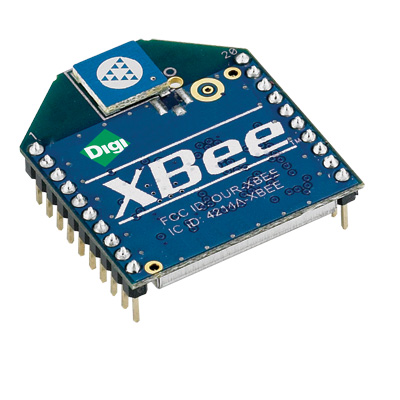
\includegraphics[scale=.16 ]{images/xBee.jpg}
 \begin{itemize}
  \item Small form factor (just larger than U.S. quarter)
  \item Low power consumption (\textasciitilde .1 W)
  \item Talk over ZigBee protocol
 \end{itemize}
}

\frame{
 \frametitle{ZigBee}
 \begin{itemize}
  \item Prototyping hardware
  \item ZigBee specification  
 \end{itemize}
}
\subsection{Server and Coordinator}

\frame{
 \frametitle{Coordinator Design}
  Must:
 \begin{itemize}
		\item Host Coordinator XBee
		\item Host LCD to display IP
		\item Listen for readings
		\item Send readings to Server
 \end{itemize}
}

\frame{
 \frametitle{Coordinator Implementation}
 Arduino:
 \begin{itemize}
	\item Talks to LCD using SoftwareSerial
	\item Listens for readings from XBee
	\item Sends readings over USB cable
 \end{itemize}
}

\frame{
 \frametitle{Server Design}
 Server must:
 \begin{itemize}
  \item Be small
  \item Consume as little power as possible
  \item Listen for readings from Coordinator 
  \item Store readings
  \item Host all of the Display
 \end{itemize}
}

\frame{
 \frametitle{Server Implementation}
  Raspberry Pi:
 \begin{itemize}
  \item Small form factor (\textasciitilde 8.5 x 5.6 cm)
  \item Low power consumption (\textasciitilde 3.5 W)
  \item Acts as data center and web server for Display
 \end{itemize}
}

\section{Software Architecture}

\frame{
 \begin{center}
  { \huge Software Architecture}
 \end{center}
}

\subsection{Overview}

\frame {
 \frametitle{Software Overview}
 \begin{itemize}
  \item Python on the backend
  \begin{enumerate}[A.]
   \item Django for the REST, HTTP stuff \cite{Web:Django}
   \item Custom python to interact with Arduino interface
  \end{enumerate}
  \item Heavy Javascript on the frontend
  \begin{enumerate}[A.]
   \item jqplot for creating graphs (jQuery included) \cite{Web:jQuery}
   \item django-compress to reduce the Javascript files to a manageable size.
   \item AngularJS for a MVC architecture that consumes the REST backend \cite{Web:AngularJS}
  \end{enumerate}
 \end{itemize}
}



\frame{
 \frametitle{Backend Overview}
 \begin{itemize}
  \item Django will be used to handle database
  \item Tastypie will be used to prototype the REST API
  \item Each functional area of the project is a Django module
  \begin{enumerate}[A.]
   \item System
   \item POW-R
   \item REST API
  \end{enumerate}
 \end{itemize}
}

\subsection{Architecture}

\frame{
 \frametitle{Backend Architecture}
 \begin{center}
  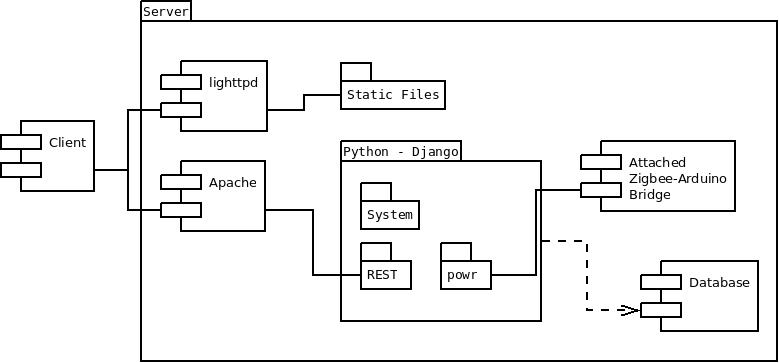
\includegraphics[width=0.8\textwidth]{Diagrams/ServerDependency.jpg}
 \end{center}
}

\frame{
 \frametitle{Frontend Architecture}
 \begin{itemize}
  \item django-compress
  \begin{enumerate}[A.]
   \item Minifies the JavaScript code so clients load faster
   \item Easy to use, can be tested
  \end{enumerate}
  \item AngularJS - MVC Architecture on the client-side
  \item jqplot - Renders charts and graphs
  \item jQuery - Deals with all the behind-the-scenes AJAX stuff
 \end{itemize}
}

\frame{
 \frametitle{Frontend Architecture}
 \begin{center}
  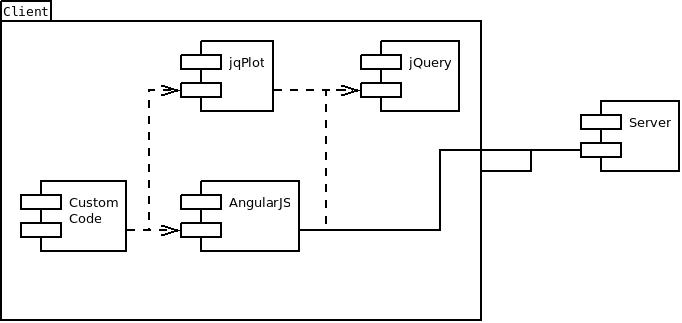
\includegraphics[width=0.8\textwidth]{Diagrams/ClientDependency.jpg}
 \end{center}
}
\section{Software Implementation}

\frame{
 \begin{center}
  { \huge Software Implementation}
 \end{center}
}

\subsection{How did things go?}

\frame {
 \frametitle{Software Implementation}
 \begin{itemize}
  \item Went more-or-less according to plan
  \begin{enumerate}
   \item We switched away from Backbone.js and iCanHaz because AngularJS covered both domains
   \item We didn't use Asynchronous Module Definition (AMD) because very few libraries supported it
   \item There were some small modifications to the REST API to make it more compatible with the world
  \end{enumerate}
  \item Biggest software problem was the complexity of the setup
  \begin{enumerate}
   \item Because of the number of libraries and frameworks, it was difficult to do development in Windows
   \item We developed two solutions; a completely isolated Python development environment, and a VirtualBox for people with Windows
  \end{enumerate}
 \end{itemize}
}

\subsection{Changes to the design}

\frame {
 \frametitle{Software Implementation}
 \begin{itemize}
  \item Some things didn't make it to the final product for a variety of reasons
  \begin{itemize}
   \item Adding satellites was ditched because it was too confusing for an end user
   \item The power-bill-guestimater was ditched because it would be impossible to accurately track all power consumption, thus leading to incorrect guestimates
   \item The user-management stuff was simplified because we don't need a complex permission system
  \end{itemize}
  \item Some things were added
  \begin{itemize}
   \item We used Intro.JS to create a "help" feature in our website
   \item We added a JS compressor to keep the codebase small when delivered to the client
  \end{itemize}
 \end{itemize}
}

\section{Testing}

\frame{
 \begin{center}
  { \huge Testing}
 \end{center}
}
 
\subsection{Test Cases}

\frame{
  \frametitle{Test Cases - Unit}
    \begin{itemize}
	  \item REST API
	  \item Unicode and Backend
	  \item Python Automated Tests
	  \item Zigbee Mesh Test
	  \item Voltage Circut Test
	  \item Current Circuit Test
	\end{itemize}
}

\frame{
  \frametitle{Test Cases - Integration}
    \begin{itemize}
	  \item Create a Graph
	  \item View Graphs
	  \item Data Retention Across Satellites
	  \item Zigbee Data Transfer
	  \item Satellite-to-Server Protocol
	\end{itemize}
}

\frame{
  \frametitle{Test Cases - System}
    \begin{itemize}
	  \item Log In
	  \item Log Out
	  \item Add Device
	  \item Disable Device
	  \item Add User
	  \item Remove User
	  \item Rename Device
	  \item Reassign Device
	\end{itemize}
}

\frame{
  \frametitle{Test Cases - Acceptance}
    \begin{itemize}
	  \item Ease of Learning
	  \item Examining the Satellite
	  \item Examining the Server
	  \item Data Loss Error
	  \item Display Responsiveness
	\end{itemize}
}

\subsection{Test Results}
 
\frame{
  \frametitle{Test Results}
    \begin{itemize}
	  \item Failed Tests:
		\begin{itemize}
			\item Ease of Learning
			\item Remove User
		\end{itemize}
	  \item Corrective Action Taken
		\begin{itemize}
			\item Edited four tests to accomodate late changes
			\item Adjusted User Management page to make "Remove User" test passable
			\item Made plans for UI changes that would allow "Ease of Learning" test to pass
		\end{itemize}
	\end{itemize}
}

\section{Closing}
\subsection{Reflection}

\frame{
 \frametitle{Lessons Learned}
	\begin{itemize}
		\item Order parts ASAP
		\item Understanding new material
		\item Team dynamics
		\item Time management
	\end{itemize}
 }

\frame{
 \frametitle{How would we do it all over again?}
    \begin{itemize}
		\item Start development sooner
		\item Stick to schedule
	\end{itemize}
}

\frame{
 \frametitle{Future plans, potential improvements}
    \begin{itemize}
		\item Satellite functionality
		\item Home Automation Framework
	\end{itemize}
}
\subsection{Demonstration}

\frame{
 \frametitle{Demonstration time!}
	\begin{center}
	{\huge Check it out!}
	\end{center}
 }

\frame{
 \frametitle{Questions and Closing}
    \begin{center}
        {\huge Questions?}
        
        {\small Presentation made using \LaTeX{} }

		
		Our website: \url{http://powr.logrit.com/}
		
    \end{center}
}

\end{document}

